\chapter{Test Cases}
\label{ch:testcases}
Each Test Case represents vertical and inclined wells with identical parameters. Currently, all Test Cases were run for off-bottom case. For Test Cases 3 and 4, we incorporated BHA to compare the outputs of the two models. Initially, all Test Cases were executed with various static and friction factor values, which are described in the subsequent subsections. However, an additional set of experiments were conducted with identical static and dynamic friction factor values. Since there is no friction in vertical wells, it is primarily related to inclined wells. The problem with the ExxonMobil model's on-bottom case has been resolved. In addition, there is an issue with mud motor that we are addressing. Regarding the Aarsnes-Shor model, since the issue with the Python version has not been resolved, Only Matlab version was used for the final results. The Python version was only executed with Test Case 1 (it will be added once the issue has been resolved). \tablename~\ref{Test_case_summary} summarizes characteristics of each Test Case. 

\begin{table}
    \centering
    \begin{tabular}{|c|c|c|c|c|c|c|}
        \hline
        \textbf{Test Cases} & \textbf{Well Type} & \textbf{Static FF} & \textbf{Dynamic FF}& \textbf{BHA}\\
        \hline
        Test Case 1 & Vertical & 0 & 0 & X\\
        \hline
        Test Case 2a & Deviated (60\textdegree{}) & 0.5 & 0.5 & X \\
        \hline
        Test Case 2b & Deviated (60\textdegree{}) & 0.5 & 0.25 & X \\
        \hline
        Test Case 3 & Vertical & 0 & 0 & O\\                                                
        \hline
        Test Case 4a & Deviated (60\textdegree{}) & 0.5 & 0.5 & O \\                                                  
        \hline
        Test Case 4b & Deviated (60\textdegree{}) & 0.5 & 0.25 & O \\                                                     
        \hline
    \end{tabular}
    \caption[Summary of characteristics of each Test Case]{Summary of characteristics of each Test Case.}
    \label{Test_case_summary}
\end{table} 


\section{Terminology}
\subsection{No BHA vs BHA}

The Test Cases in this study focus on comparing drilling scenarios with and without the Bottom Hole Assembly (BHA). It introduces specific parameters that differ from the rest of the drill pipe in terms of weight and diameter. However, when the BHA is not present, that particular section of the drill pipe above the bit will have the same weight and diameter as the rest of the drill pipe.

To maintain simplicity and establish a baseline, we begin the study with a single drill pipe configuration. This configuration represents the most straightforward drilling arrangement, with a solitary pipe running from the surface to the drill bit. In this case, the weight and diameter of the entire drill pipe, including the section above the bit, are uniform.

As we proceed with the investigation, we will introduce the BHA into the system and examine its impact on drilling dynamics. The BHA's distinct parameters, such as its weight and diameter, will be considered in the analysis to understand how it influences drilling performance. By conducting these comparative analyses, we aim to gain valuable insights into the effects of the BHA on the drill string's behavior and the overall drilling process.

In the next subsection we will explore additional configurations with varying BHA designs and properties to further investigate their influence on drilling efficiency and performance. These test cases will enable us to optimize drilling operations and develop a comprehensive understanding of how the presence or absence of the BHA affects the system's behavior.

\subsection{Different vs Same FF}

Both models under consideration account for both static and dynamic friction factors (FF), but the disparity in FF values is expected to be more pronounced in inclined wells compared to vertical ones. To gain insights into the impact of varying and consistent FF values on drilling dynamics, a detailed investigation is warranted.

In inclined wells, the interaction between the drill string and the wellbore wall becomes more complex due to the influence of gravity and the inclination angle. This results in differing frictional forces acting on the drill string as it traverses the wellbore. As a consequence, the FF values play a crucial role in affecting the drilling performance and behavior.

\section{Test Case 1 - Vertical well, No BHA}
The model parameters and schematic of the wellbore surveys and drill string components are shown in Table \tablename~\ref{table_verticalwell_input} and \ref{figure_verticalwell}. The ExxonMobil model and MATLAB ver.\ A-S model uses metric units while PYTHON ver.\ A-S model uses imperial units. For the future convenience, the tables in this chapter contains both imperial and metric units.

\begin{figure}[!hbt]
  \centering
  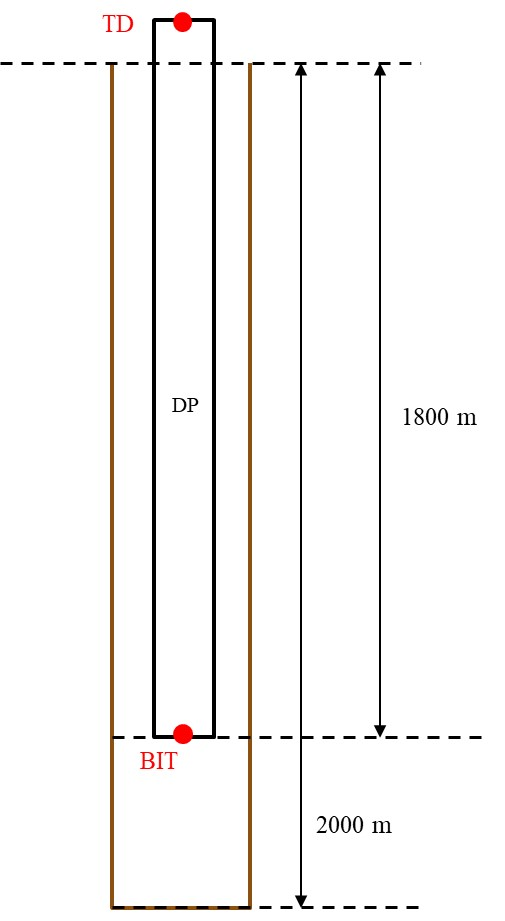
\includegraphics[width=1.5in]{VerticalWellConfig}
  \caption[Schematic of well and drill string for model comparison.]{Schematic of well and drill string for model comparison.}\label{figure_verticalwell}
\end{figure}

\begin{testcasetable}
$\rho$ & 490.6 $lb/ft^3$ & 7850 $kg/m^3$ & Drill pipe density \\                                                  
\hline
G & 1.67$\cdot$10$^{9}$ $lbf/ft^2$ & 7.99$\cdot$10$^{10}$ $Pa$  & Shear modulus \\                                                  
\hline
OD & 5.88 $in$ & 0.15 $m$ & Drill pipe outer diameter\\                                                       
\hline
ID & 5.00 $in$ & 0.127 $m$ & Drill pipe inner diameter  \\                                                      
\hline
MD & 6561 $ft$ & 2000 $m$ & Measured depth\\                                                              
\hline
TVD & 6561 $ft$ & 2000 $m$ & Total vertical depth\\
\hline
Bit depth & 5905 $ft$ & 1800 $m$ & - \\ 
\hline
\end{tabularx}
\caption[Well survey data for model comparison (vertical well)]{Well survey and drill string data for model comparison (vertical well without BHA components)}\label{table_verticalwell_input}
\end{testcasetable}
The test was conducted by assuming the top drive velocity to be increased from 0 $RPM$ to 40 $RPM$ at 1 second and maintained the velocity for rest of the time. The top drive velocity is shown in \figurename~\ref{figure_topdrive_VSP}

\begin{figure}[!hbt]
  \centering
  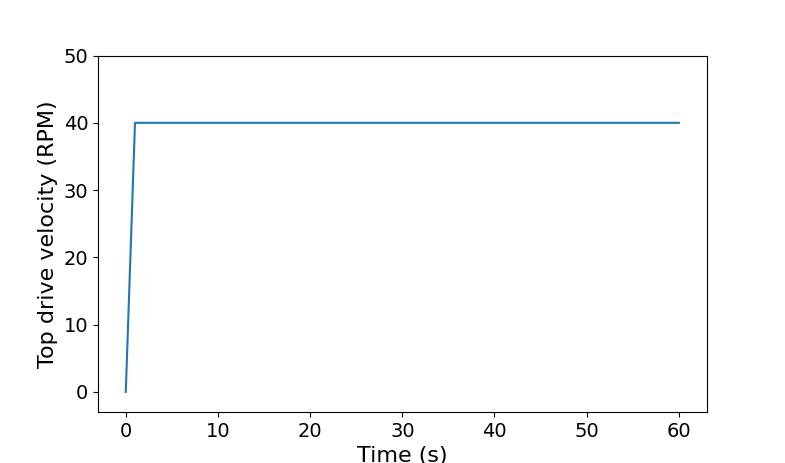
\includegraphics[width=3in]{TopdriveVSP}
  \caption[Top drive set velocity]{Top drive set velocity}\label{figure_topdrive_VSP}
\end{figure}

\section{Test Case 2 - Inclined well, No BHA}
\subsection{Test case 2a - Same FF values}
The models were tested with inclined well with simple configuration of drill string. The MD of the well is 4000 $m$ with 60$^{\circ}$ inclination. The drill bit is off-bottom where located at 2500 $m$ depth. The Schematic view of wellbore and drill string are depicted in \figurename~\ref{figure_wellconfig_inclined}. Also, the top drive velocity is increased to 40 $RPM$ at 1 second which is same with Test Case 1 (\figurename\ref{figure_topdrive_VSP}). For Test Case 2, the viscous damping is neglected for the simplicity of the test. However, Coulomb friction is considered to investigate the stick-slip occurrence during drilling. The parameters for the test are summarized in \tablename~\ref{table_Inclinedwell_2a_input}.

\begin{figure}[!hbt]
  \centering
  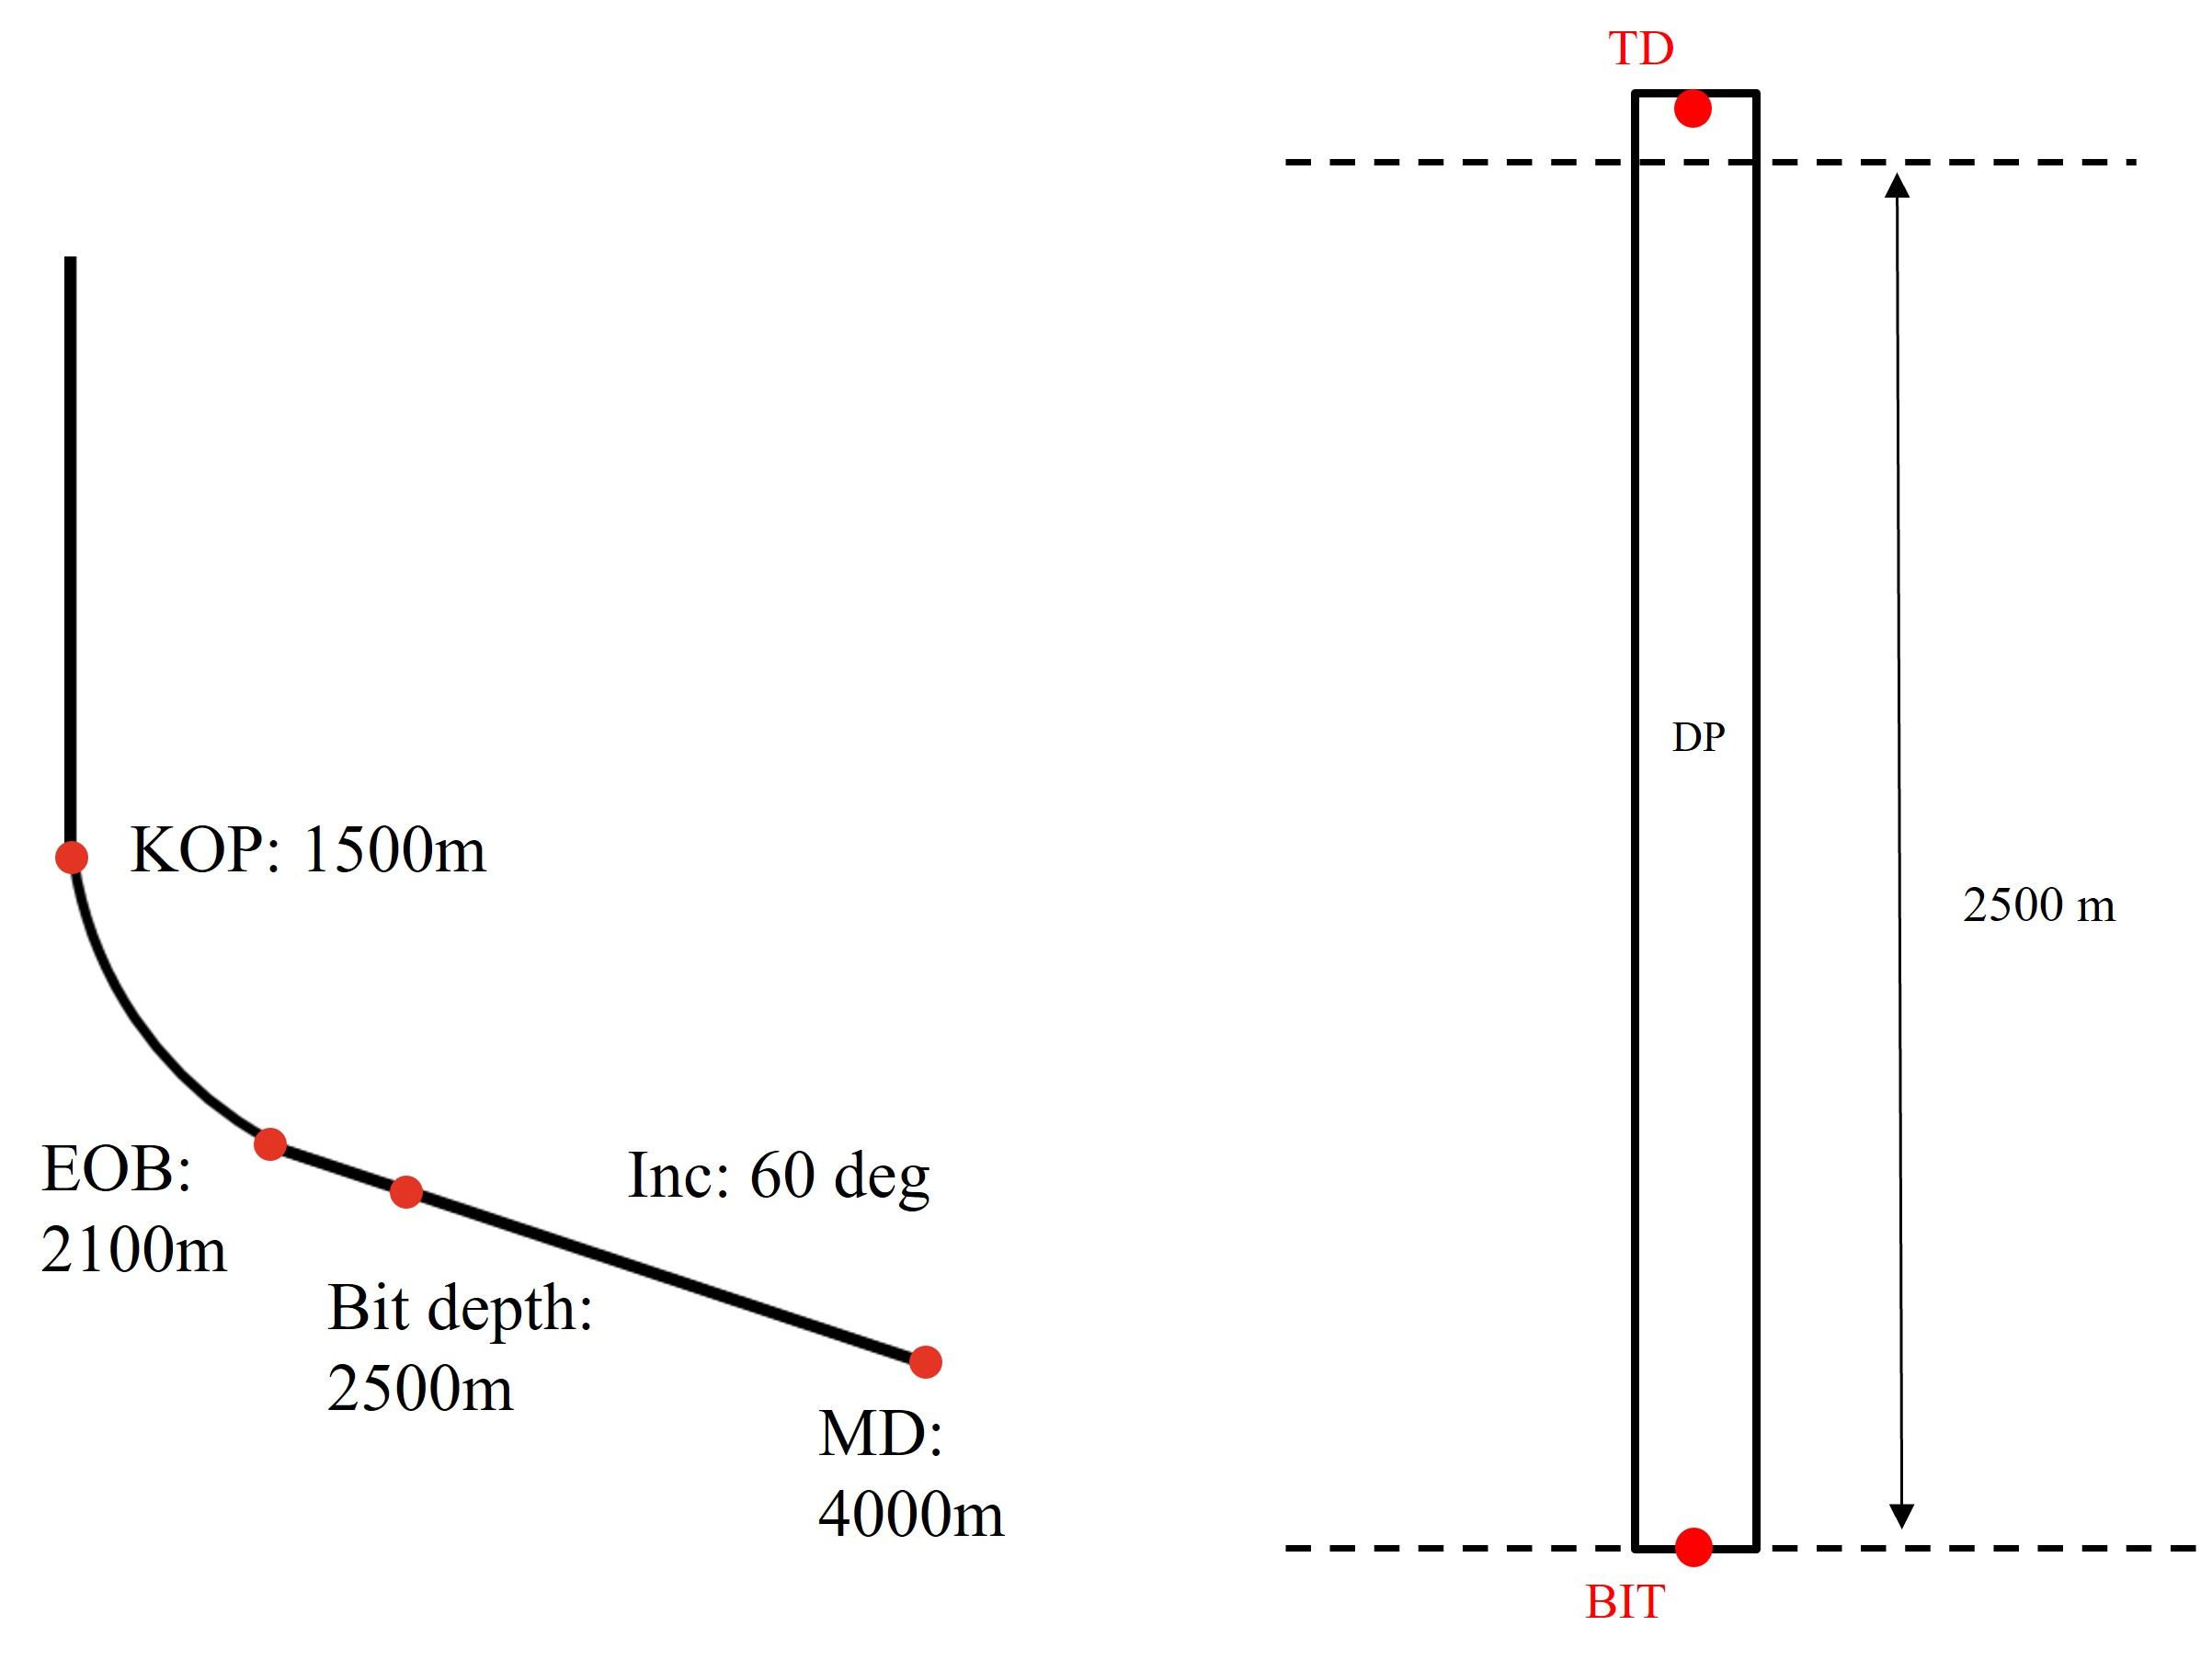
\includegraphics[width=4in]{InclinedWellConfig}
  \caption[Schematic view of Test Case 2.]{Schematic view of wellbore and drill string for Test Case 2.}\label{figure_wellconfig_inclined}
\end{figure}

\begin{testcasetable}
  $OD_{dp}$ & 5.88 $in$ & 0.15 $m$ & Drill pipe outer diameter\\                                                       
  \hline
  $ID_{dp}$ & 5.00 $in$ & 0.127 $m$ & Drill pipe inner diameter  \\                                                      
  \hline
  $\rho_{dp}$ & 490.6 $lb/ft^3$ & 7850 $kg/m^3$ & Drill pipe density \\                                                  
  \hline
  $G_{dp}$ & 1.27$\cdot$10$^{9}$ $lb/ft^2$ & 6.10$\cdot$10$^{10}$ $Pa$ & Drill pipe shear modulus\\                                                              
  \hline
  $\mu_{s}$ & 0.5 & 0.5 & Static friction factor\\
  \hline
  $\mu_{d}$ & 0.5 & 0.5 & Dynamic friction factor\\
  \hline
  $w_c$ & 10 $RPM$ & 10 $RPM$ & Cut-off angular velocity\\
  \hline
  $\theta$ & 60$^{\circ}$ & 60$^{\circ}$ & Inclination\\
  \hline
  \end{tabularx}
\caption[Input parameters for Test Case 2a]{Input parameters for Test Case 2a.}\label{table_Inclinedwell_2a_input}
\end{testcasetable}

\subsection{Test Case 2b - Different FF values}
The models were tested with the exact same configuration from the previous subsection, except different values of static and dynamic FF values. The following \tablename~\ref{table_Inclinedwell_2b_input} summarizes the input parameters. 

\begin{testcasetable}
   $OD_{dp}$ & 5.88 $in$ & 0.15 $m$ & Drill pipe outer diameter\\                                                       
   \hline
   $ID_{dp}$ & 5.00 $in$ & 0.127 $m$ & Drill pipe inner diameter  \\                                                      
   \hline
   $\rho_{dp}$ & 490.6 $lb/ft^3$ & 7850 $kg/m^3$ & Drill pipe density \\                                                  
   \hline
   $G_{dp}$ & 1.27$\cdot$10$^{9}$ $lb/ft^2$ & 6.10$\cdot$10$^{10}$ $Pa$ & Drill pipe shear modulus\\                                                              
   \hline
   $\mu_{s}$ & 0.5 & 0.5 & Static friction factor\\
   \hline
   $\mu_{d}$ & 0.25 & 0.25 & Dynamic friction factor\\
   \hline
   $w_c$ & 10 $RPM$ & 10 $RPM$ & Cut-off angular velocity\\
   \hline
   $\theta$ & 60$^{\circ}$ & 60$^{\circ}$ & Inclination\\
   \hline
\end{tabularx}
\caption[Input parameters for Test Case 2b]{Input parameters for Test Case 2b.}\label{table_Inclinedwell_2b_input}
\end{testcasetable}

\section{Test Case 3 - Vertical Well with BHA}
In this specific scenario, an additional configuration of the drill string included BHA. The BHA introduced extra components, resulting in an increase in both the weight and size of the drill string. However, the well survey data for the vertical well remained the same, except for the incorporation of the BHA. The well design, depicted in \figurename~\ref{Vert_well_conf_BHA}, remained unchanged, as well as, the parameters for the top drive. For the sake of simplicity, the influence of viscous damping was disregarded. The specific input parameters can be found in the \tablename~\ref{Input Parameters TC3}.

\begin{figure}
  \centering
  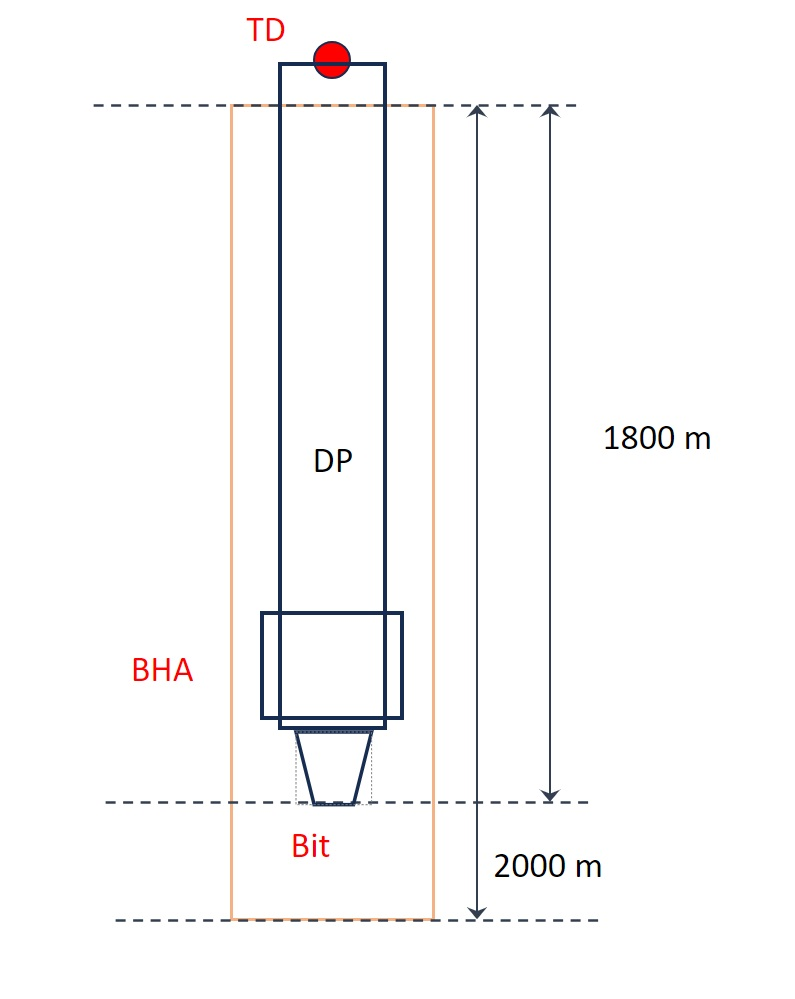
\includegraphics[width=2in]{VerticalWellConfigBHA}
  \caption{Schematic of well and drill string for model comparison}\label{Vert_well_conf_BHA}
\end{figure}


\begin{testcasetable}
    $OD_{HWDP}$ & 4.50 $in$ & 0.1143 $m$ & Heavy weight drill pipe outer diameter \\
    \hline
    $ID_{HWDP}$ & 2.50 $in$ & 0.0635 $m$ & Heavy weight drill pipe inner diameter \\
    \hline
    $OD_{DC}$ & 6.00 $in$ & 0.1524 $m$ & Drill collars outer diameter \\
    \hline
    $ID_{DC}$ & 2.00 $in$ & 0.0508 $m$ & Drill collars inner diameter \\
    \hline
    $L_{HWDP}$ & 60 $ft$ & 18.30 $m$ & Length of heavy weight drill pipe \\
    \hline
    $L_{DC}$ & 270 $ft$ & 82.30 $m$ & Length of drill collars \\
    \hline
    $\rho_{dp}$ & 490.6 $lb/ft^{3}$ & 7850 $kg/m^{3}$ & Drill pipe density \\
    \hline
    $G_{dp}$ & 1.67$\cdot$10$^{9}$ $lb/ft^2$ & 7.99$\cdot$10$^{10}$ $Pa$ & Drill pipe shear modulus\\  
    \hline
    \end{tabularx}
  \caption{Input parameters of BHA for Test Case 3}\label{Input Parameters TC3}
\end{testcasetable} 

\section{Test Case 4 - Inclined Well with BHA}
\subsection{Test Case 4a - Same FF values}

The models were tested with the same input parameters from Test Case 2, with additional configuration of the drill string including BHA. Well survey data for the inclined well remained same, except for the incorporation of the BHA. The well design, depicted in \figurename~\ref{figure_wellconfig_inclined_BHA}, remained unchanged, as well as, the parameters for the top drive. As stated previously in Test Case 2 the influence of viscous damping was disregarded. The input parameters can be found in the  \tablename~\ref{table_Inclinedwell_4a_input}.

\begin{figure}[!hbt]
  \centering
  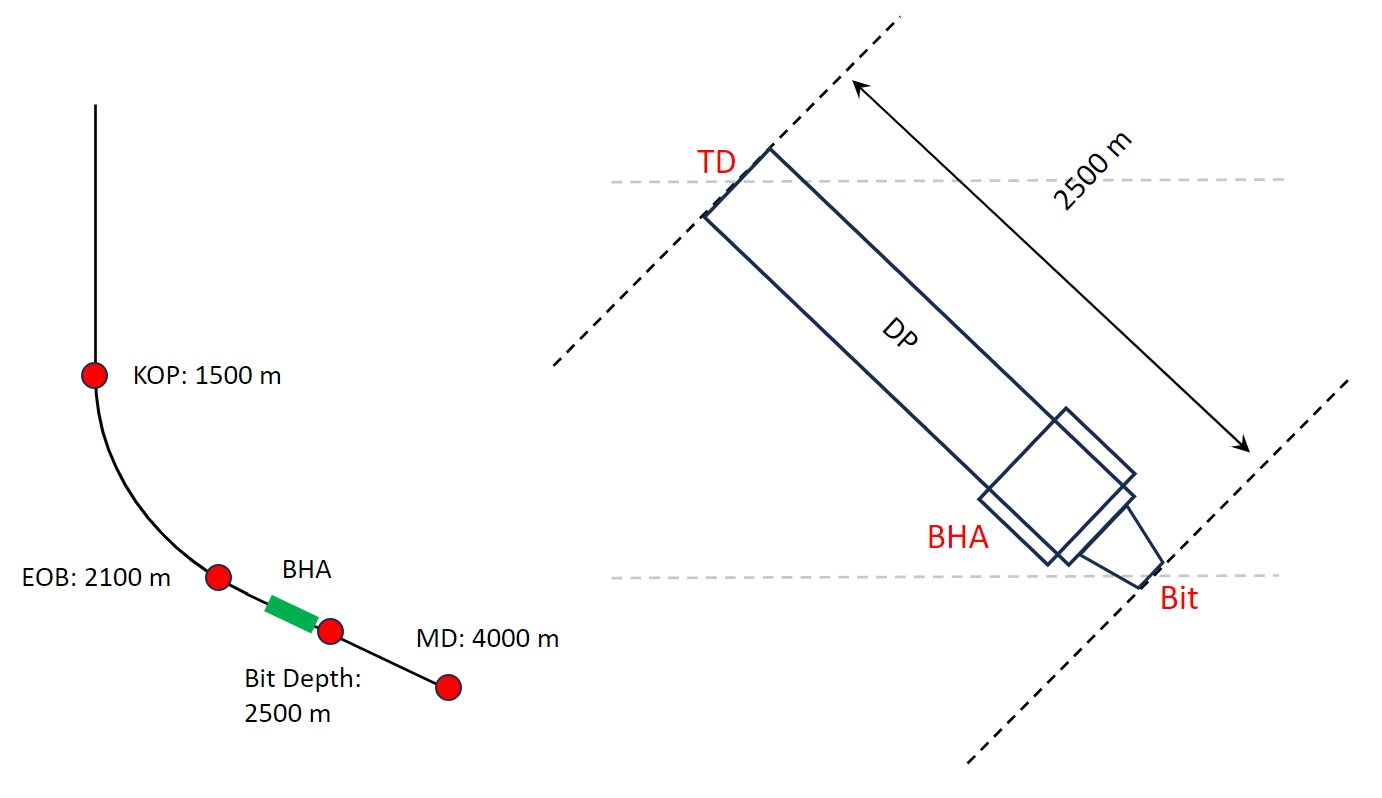
\includegraphics[width=4in]{InclinedWellConfigBHA}
  \caption[Schematic view of Test Case 4.]{Schematic view of wellbore and drill string for Test Case 4.}\label{figure_wellconfig_inclined_BHA}
\end{figure}

\begin{testcasetable}
   $OD_{HWDP}$ & 4.50 $in$ & 0.1143 $m$ & Heavy weight drill pipe outer diameter \\
   \hline
   $ID_{HWDP}$ & 2.50 $in$ & 0.0635 $m$ & Heavy weight drill pipe inner diameter \\
   \hline
   $OD_{DC}$ & 6.00 $in$ & 0.1524 $m$ & Drill collars outer diameter \\
   \hline
   $ID_{DC}$ & 2.00 $in$ & 0.0508 $m$ & Drill collars inner diameter \\                                                    
   \hline
   $L_{HWDP}$ & 60 $ft$ & 18.30 $m$ & Length of heavy weight drill pipe \\
   \hline
   $L_{DC}$ & 270 $ft$ & 82.30 $m$ & Length of drill collars \\
   \hline
   $\rho_{dp}$ & 490.6 $lb/ft^3$ & 7850 $kg/m^3$ & Drill pipe density \\                                                  
   \hline
   $G_{dp}$ & 1.27$\cdot$10$^{9}$ $lb/ft^2$ & 6.10$\cdot$10$^{10}$ $Pa$ & Drill pipe shear modulus\\  
   \hline
   $\mu_{s}$ & 0.5 & 0.5 & Static friction factor\\
   \hline
   $\mu_{d}$ & 0.5 & 0.5 & Dynamic friction factor\\
   \hline
   $w_c$ & 10 $RPM$ & 10 $RPM$ & Cut-off angular velocity\\
   \hline
   $\theta$ & 60$^{\circ}$ & 60$^{\circ}$ & Inclination\\
   \hline
   \end{tabularx}
   \caption[Input parameters for Test Case 4a]{Input parameters for Test Case 4a.}\label{table_Inclinedwell_4a_input}
\end{testcasetable}

\subsection{Test Case 4b - Same Friction Factor values}

Lastly, the models were tested with the exact same configuration from the previous subsection, except with different values of static and dynamic FF values. The following \tablename~\ref{table_Inclinedwell_4b_input} summarizes the input parameters. 

\begin{testcasetable}
   $OD_{HWDP}$ & 4.50 $in$ & 0.1143 $m$ & Heavy weight drill pipe outer diameter \\
   \hline
   $ID_{HWDP}$ & 2.50 $in$ & 0.0635 $m$ & Heavy weight drill pipe inner diameter \\
   \hline
   $OD_{DC}$ & 6.00 $in$ & 0.1524 $m$ & Drill collars outer diameter \\
   \hline
   $ID_{DC}$ & 2.00 $in$ & 0.0508 $m$ & Drill collars inner diameter \\                                                    
   \hline
   $L_{HWDP}$ & 60 $ft$ & 18.30 $m$ & Length of heavy weight drill pipe \\
   \hline
   $L_{DC}$ & 270 $ft$ & 82.30 $m$ & Length of drill collars \\
   \hline
   $\rho_{dp}$ & 490.6 $lb/ft^3$ & 7850 $kg/m^3$ & Drill pipe density \\                                                  
   \hline
   $G_{dp}$ & 1.27$\cdot$10$^{9}$ $lb/ft^2$ & 6.10$\cdot$10$^{10}$ $Pa$ & Drill pipe shear modulus\\                                                                
   \hline
   $\mu_{s}$ & 0.5 & 0.5 & Static friction factor\\
   \hline
   $\mu_{d}$ & 0.25 & 0.25 & Dynamic friction factor\\
   \hline
   $w_c$ & 10 $RPM$ & 10 $RPM$ & Cut-off angular velocity\\
   \hline
   $\theta$ & 60$^{\circ}$ & 60$^{\circ}$ & Inclination\\
   \hline
   \end{tabularx}
\caption[Input parameters for Test Case 4b.]{Input parameters for Test Case 4b.}\label{table_Inclinedwell_4b_input}
\end{testcasetable}
